\documentclass{standalone}
\usepackage[T1]{fontenc}
\usepackage[latin2]{inputenc}
\usepackage[english]{babel}
\usepackage{tikz}
\usetikzlibrary{calc,through,backgrounds,positioning,fit}
\usetikzlibrary{shapes,arrows,shadows}
\usetikzlibrary{calendar}
\tikzstyle{stt}=[shape=circle, draw, minimum height=6mm]
\begin{document}
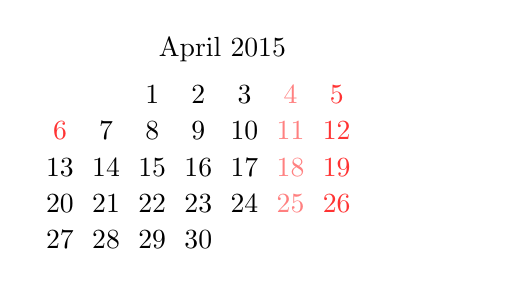
\begin{tikzpicture}
[matrix of nodes/.style={
	execute at begin cell=\node\bgroup,
	execute at end cell=\egroup;%
},
row 2 column 1/.style={red!80},
column 6/.style={red!50},
column 7/.style={red!80}]

\node [text width=4cm] at (1.5,1.5) {April 2015};
\matrix[matrix of nodes]
{
	 &  &  1 & 2 & 3 & 4 & 5\\
6& 7  &  8 & 9 & 10 & 11 & 12\\
13& 14 &  15 & 16 & 17 & 18 & 19\\
20&  21&  22 & 23 & 24 & 25 & 26\\
27&28  &  29 & 30 &  &  & \\
};
 
\end{tikzpicture}
\end{document}